%%%% Case study section


\section{Case Study}

%% paragraph 1 -- experimental environment
This section reports our case study performing real-time monitoring of a CAN network for realistic safety properties. We have implemented the \monitor algorithm on a low cost ARM-Cortex M4 development board which can be used to monitor CAN networks. For this case study we have obtained CAN network logs from a series of robustness tests on an autonomous research vehicle which we have replayed on a test CAN bus for the monitor to check. This setup is shown in Figure \ref{fig:replaySchem}.

\begin{figure}
\centering
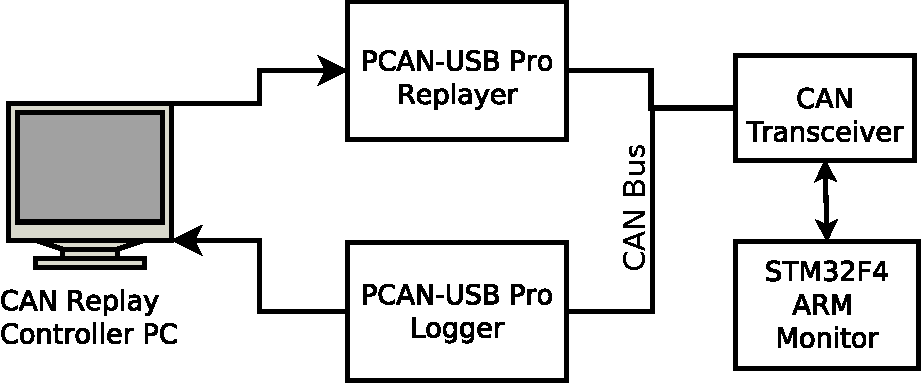
\includegraphics[width=4.5in]{img/replay_arch}
\caption{CAN replay network setup \label{fig:replaySchem}}
\end{figure}

%% paragraph 2 -- experiment goal
We wish to use the CAN monitor to check a realistic set of safety policies over a real network trace. From this, we can see the feasibility of performing external bus monitoring for these types of systems.

%% paragraph 3 -- description of experiment 
%%% some of this is in para1, we should go over: specification, logs, etc
The logs contain both normal operation as well as some operation under network-based robustness testing. During robustness testing, the testing framework can hijack targeted network messages on the bus to inject testing values. % could cite astaa here
A PC was connected to a PCAN-USB Pro \cite{PCAN-USBPro} device which provides a USB interface to two CAN connections. One CAN channel was used as the log replayer, while the other was used as a bus logger for analysis purposes.

%% paragraph 4 -- specification
Requirements documentation for this system was available, so we were able to build a monitoring specification based on actual system requirements.
The specification evaluated in the embedded monitor on the test logs are shown in Table \ref{tab:monspec}. This specification was derived from the system requirements based on the observable system state available in the testing logs. 


Rule \#0 is a heartbeat detection which ensures that the interface component is still running (essentially a watchdog message). Rule \#1 is a second component of this check. The system's heartbeat message contains a single heartbeat status bit which we checked directly in Rule \#0, but the message also has a rolling counter field. We use the system interface to ensure that this counter is correct, and check the system interface's output ($\pred{HeartbeatOk}$) in Rule \#1.
We also checked for illegal state transitions. Rules \#2 through \#5 check both for illegal transition commands and actual illegal state transitions.

\begin{table}
%\begin{tabular}{|p{3in}|l|}
\begin{tabular}{|l|p{4.5in}|}
\hline \multirow{2}{*}{Rule \#} & Informal Rule \\ & BMTL \\
\hline \multirow{2}{*}{0} & A feature heartbeat shall be received every 500ms \\
& $\pred{HeartbeatOn} \rightarrow \lozenge_{[0,500ms]} \pred{HeartBeat}$ \\
\hline \multirow{2}{*}{1} & The interface component heartbeat counter is correct \\
& $\pred{HeartbeatOn} \rightarrow \pred{HeartbeatCounterOk}$ \\
\hline \multirow{2}{*}{2} & The vehicle shall not transition from manual mode to autonomous mode \\
&  $\neg ((\blacksquare_{[1,1]} \pred{IntManualState}) \wedge \pred{IntAutoStat})$\\
\hline \multirow{2}{*}{3} & The vehicle controller shall not command a transition from manual mode to autonomous mode \\
& $\neg ((\blacksquare_{[1,1]} \pred{VehManualModeCmd}) \wedge \pred{VehAutoModeCmd})$\\
\hline \multirow{2}{*}{4} & The vehicle shall not transition from system off mode to autonomous mode \\ 
&  $\neg ((\blacksquare_{[1,1]} \pred{IntSDState}) \wedge \pred{IntAutoStat})$\\
\hline \multirow{2}{*}{5} & The vehicle controller shall not command a transition from system off mode to autonomous mode \\
& $\neg ((\blacksquare_{[1,1]} \pred{VehSDModeCmd}) \wedge \pred{VehAutoModeCmd})$\\
% warn was at 200ms
\hline
\end{tabular}
\caption{Case study monitoring specification \label{tab:monspec}}
\end{table}

\subsection{Monitoring Results}
Monitoring the test logs with the above specification resulted in identifying two real violations as well as some false positive violation detections caused by the testing infrastructure.

% covering all three possible violation types. One was a false positive
Three different types of heartbeat violations were identified after inspecting the monitor results.
% missing hb message
The first is a late heartbeat message. In one of the robustness testing logs the heartbeat message was not sent on time, which is clearly a heartbeat violation. Figure \ref{fig:hb_arrival} shows the heartbeat counter values and the inter-arrival time of the heartbeat messages over time for this violation. We can see here that the heartbeat counter did in fact increment in a valid way, just too slowly. 

\begin{figure}
		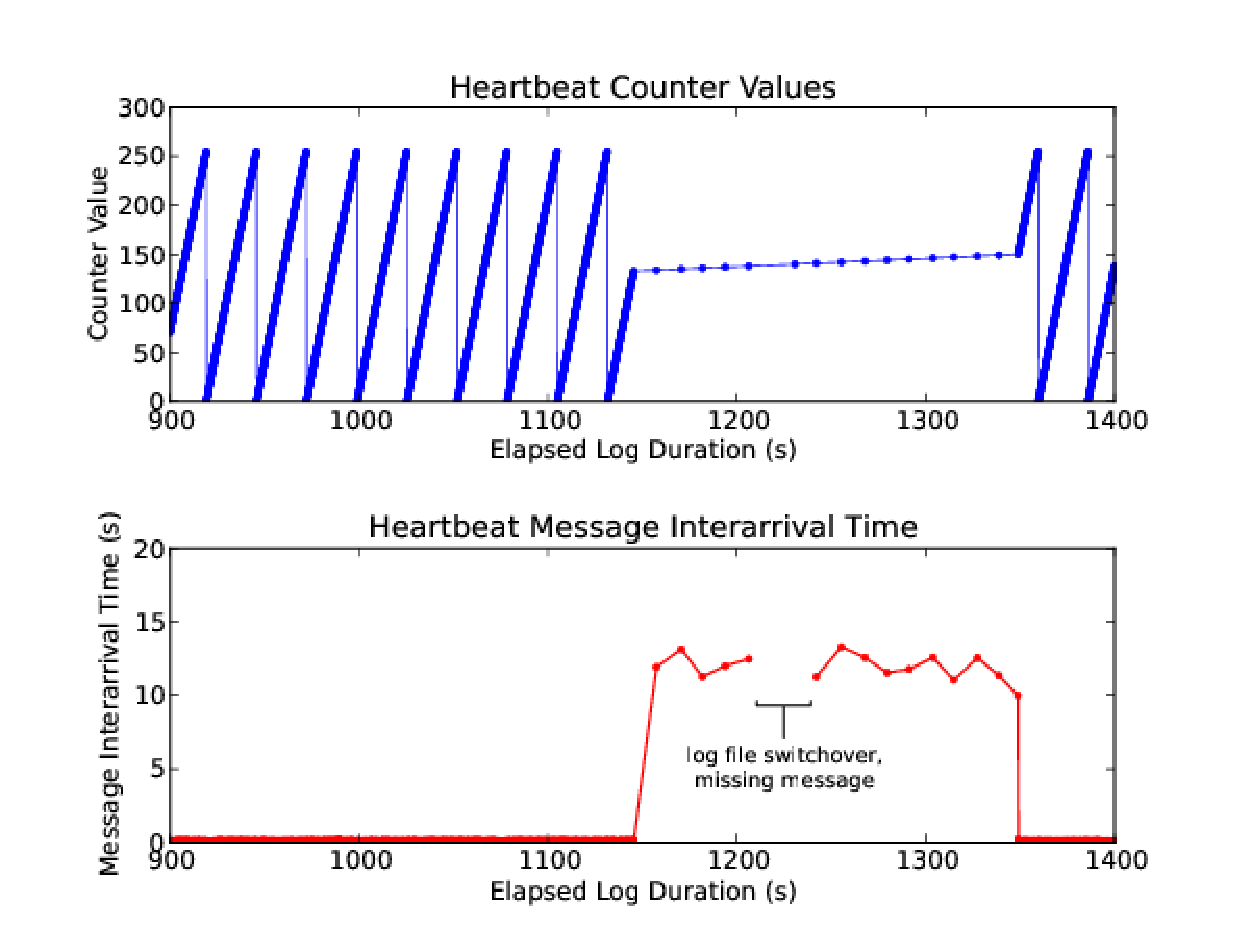
\includegraphics[width=4.5in]{img/hb1}
		\caption{Heartbeat counter values over time}
		\label{fig:hb_arrival}
\end{figure}

% bad status
The second violation is on-time heartbeat status message but the heartbeat status field is 0. 
We do not know from the available documentation whether a bad status in an on-time message with a good counter is valid or not. So without more information we cannot tell whether these violations are false positives or not. This is worthy of further investigation.

% bad counter
The last type of violation is a bad counter. 
We have defined a good counter as one which increments by one every message up to its maximum (255 in this case) before wrapping back to zero.
Every consecutive heartbeat status message must have an incremented heartbeat counter or a violation will be triggered. Figure \ref{fig:hb_badcounter} shows the counter value history for one of the traces with a heartbeat violation caused by a bad counter value.
%
%@EDIT describe robustness testing, define these false positives like the talk?
Further inspection of this violation showed that the bad counter values were sent by the testing framework rather than the actual system. In this case, the network traffic the monitor is seeing is not real system state but actually it is messages being injected by the testing framework. This is not a real violation (since the violating state is not the actual system state), and so we consider this a false positive violation.


\begin{figure}
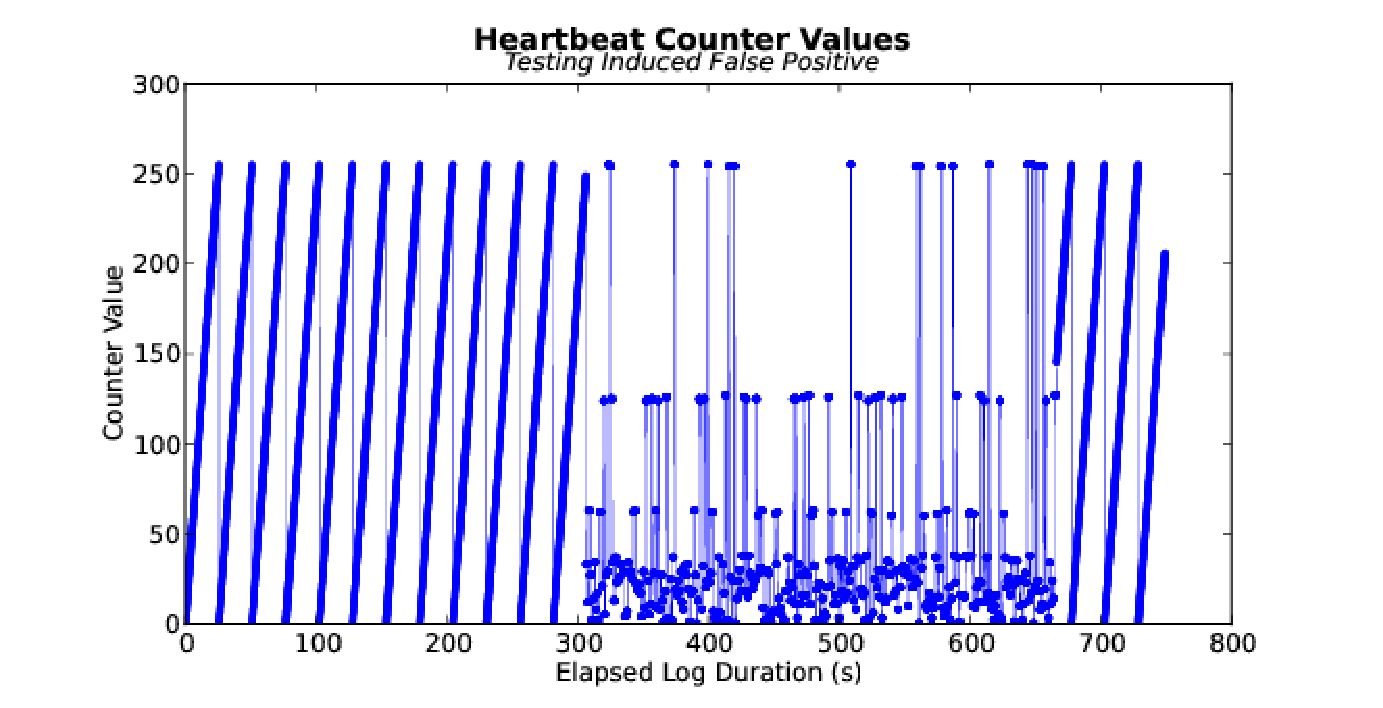
\includegraphics[width=4.5in]{img/hb2}
\caption{Bad heartbeat counter values \label{fig:hb_badcounter}}
\end{figure}

The monitor also reported violations of the legal transition rules, but these, similar to the heartbeat counter violation, also turned out to be false positives triggered by message injections by the robustness testing harness. Since the monitor checks network state, if we perform testing that directly affects the values seen on the network (such as injection/interception of network messages) we may detect violations which are created by the testing framework rather than the system. 
Information about the test configurations can be used to filter out these types of false positives which arise from test-controlled state.
This type of filtering can be automated if the test information can be input to the monitor, either directly on the network (e.g., adding a message value to injected messages) or through a side-channel (i.e., building a testing-aware monitor).
